% !TEX root = CartaPerali_Report.tex

\section{Results}
\label{sec:results}

\noindent Regardless of the deployed architecture, we noticed that normalizing our data after computing the MFCC coefficients, the training process gets stuck at a very low accuracy. The model seems to predict always a very small subset of labels regardless of the input data. The reason why this happens is because such normalization discards some important information that is instead necessary to best represent the input audio signal.

\subsection{\textbf{CNN}}
The first tested model's results are provided in Table \ref{table:cnn_performances}:\\
\begin{table}[h!]
\centering
\begin{tabular}{ p{1.5cm}|p{1.5cm}|p{1.5cm}| }
 \hline
   & Loss & Accuracy\\
\hline
Config 1 & 0\% & 100\%  \\
Config 2 & 0\% & 100\% \\
\hline
\end{tabular}
\caption{CNN Performances}
\label{table:cnn_performances}
\end{table}

\begin{figure}[h]
			\centering
	    	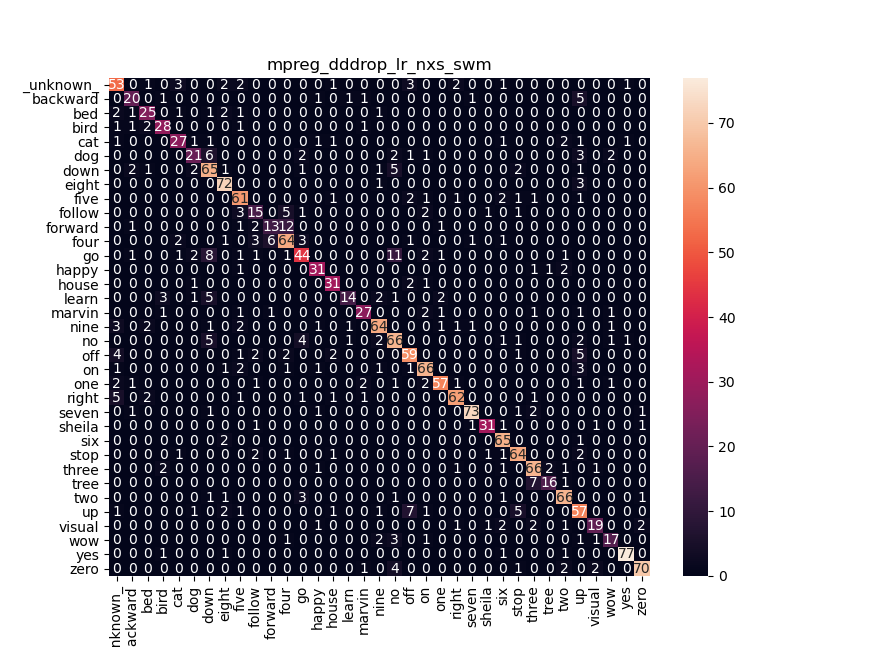
\includegraphics[width=10cm, height=8cm]{conf_matrix_cnn_dii_cm}
	    	\caption{CNN - Confusion matrix}
	    	\label{fig:conf_matrix_cnn}
\end{figure} 



\subsection{\textbf{RNN}}
The first tested model's results are provided in Table \ref{table:rnn_performances}:\\
\begin{table}[h!]
\centering
\begin{tabular}{ p{1.5cm}|p{1.5cm}|p{1.5cm}| }
 \hline
   & Loss & Accuracy\\
\hline
Config 1 & 0\% & 100\%  \\
Config 2 & 0\% & 100\% \\
\hline
\end{tabular}
\caption{RNN Performances}
\label{table:rnn_performances}
\end{table}

\begin{figure}[h]
			\centering
	    	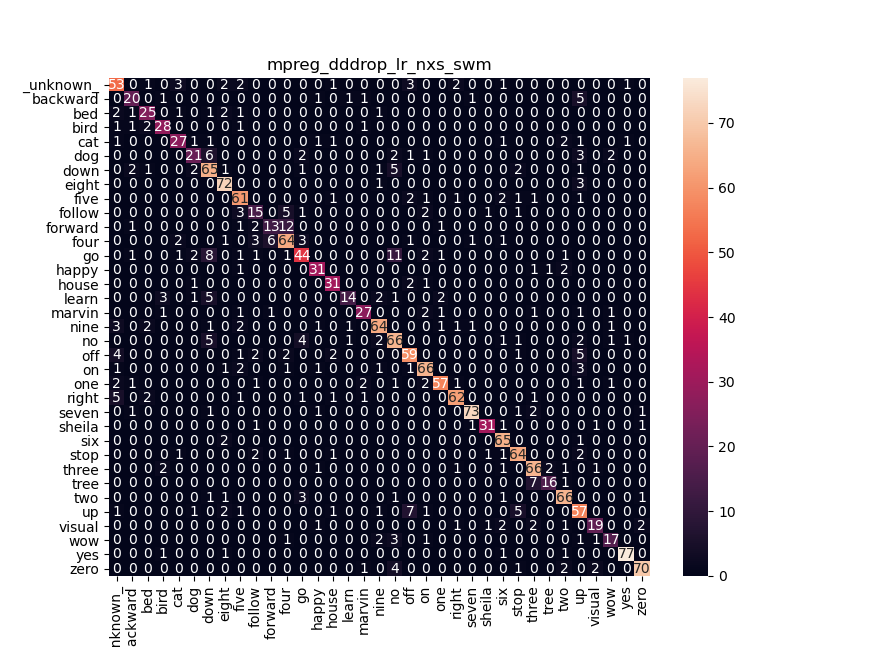
\includegraphics[width=10cm, height=8cm]{conf_matrix_cnn_dii_cm}
	    	\caption{RNN - Confusion matrix}
	    	\label{fig:conf_matrix_cnn}
\end{figure} 



\subsection{\textbf{HMM}}
The first tested model's results are provided in Table \ref{table:hmm_performances}:\\
\begin{table}[h!]
\centering
\begin{tabular}{ p{1.5cm}|p{1.5cm}|p{1.5cm}| }
 \hline
   & Loss & Accuracy\\
\hline
Config 1 & 0\% & 100\%  \\
Config 2 & 0\% & 100\% \\
\hline
\end{tabular}
\caption{HMM Performances}
\label{table:hmm_performances}
\end{table}

\begin{figure}[h]
			\centering
	    	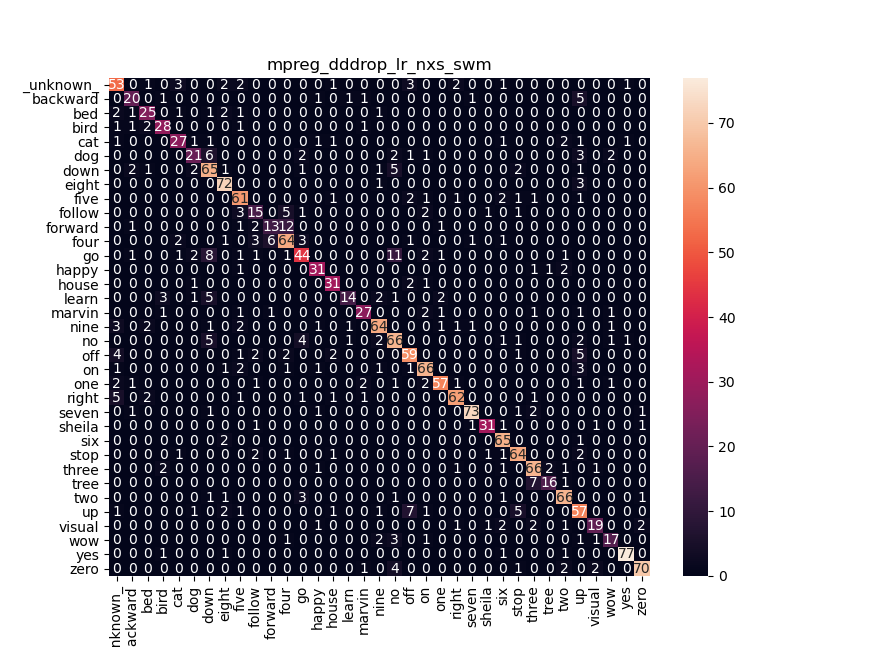
\includegraphics[width=10cm, height=8cm]{conf_matrix_cnn_dii_cm}
	    	\caption{HMM - Confusion matrix}
	    	\label{fig:conf_matrix_cnn}
\end{figure} 


\subsection*{\textbf{Models Comparisons}}
The models are compared in Table \ref{table:comparisons}:\\
\begin{table}[h!]
\centering
\begin{tabular}{ p{1.5cm}|p{1.5cm}|p{1.5cm}|p{1.5cm} }
 \hline
  & Memory & Time & Parameters \\
\hline\hline
CNN & 100\% & A & B \\
\hline
RNN & 100\% & B  & B\\
\hline
HMM &100\% & B  & B\\
\hline
\end{tabular}
\caption{Models comparisons}
\label{table:comparisons}
\end{table}\\
\noindent From the above results we can observe how {\red{to be continued...}}